\chapter{DevOps and Deployment}
\section{Environments}
\begin{longtable}{@{}p{3cm} p{5cm} p{6cm}@{}}
\toprule
\textbf{Environment} & \textbf{Purpose} & \textbf{Notes} \\
\midrule
\endhead
Local & Developer laptop & Docker Desktop, .env.local, seeded DB \\
Staging & Pre-prod test & Shared Redis/Mongo, restricted network \\
Production & End users & Auto-scaling workers, backups, observability \\
\bottomrule
\end{longtable}

\section{CI/CD}
\begin{itemize}
  \item Lint and typecheck on PR
  \item Run API and integration tests
  \item Build Next.js app and Docker base images
  \item Deploy via container orchestrator
\end{itemize}

\section{Infrastructure Diagram}
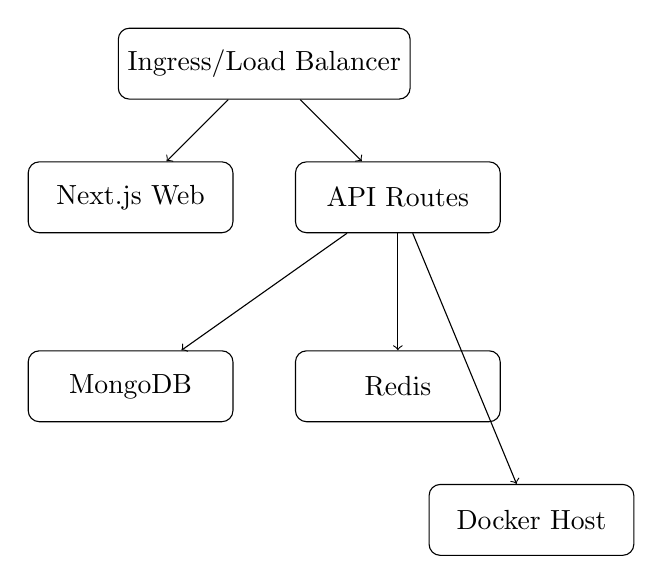
\begin{tikzpicture}[node distance=2.4cm, auto]
  \tikzstyle{svc}=[rectangle, draw, rounded corners, minimum width=2.6cm, minimum height=0.9cm]
  \node[svc] (lb) {Ingress/Load Balancer};
  \node[svc, below left of=lb] (web) {Next.js Web};
  \node[svc, below right of=lb] (api) {API Routes};
  \node[svc, below of=api] (redis) {Redis};
  \node[svc, below of=web] (mongo) {MongoDB};
  \node[svc, below right of=redis] (docker) {Docker Host};
  \draw[->] (lb) -- (web);
  \draw[->] (lb) -- (api);
  \draw[->] (api) -- (redis);
  \draw[->] (api) -- (mongo);
  \draw[->] (api) -- (docker);
\end{tikzpicture}
